% Provenance (never printed): old terminale S material on the transformation of
% rocks in mountain belts and subduction zones (pressure, temperature, index
% minerals and the Al2SiO5 polymorphs, foliation, contact and regional
% metamorphism). Owner (Sync 0): metamorphism, lithostatic pressure, polymorph,
% index mineral/isograd/metamorphic grade, foliation/schistosity, contact and
% regional metamorphism/aureole. Blueschist and eclogite are g11.06's, the
% geotherm g11.03's, minerals and silicates g11.07's, the rock families, marble
% and slate Book 1's (g6), pressure physics': recalled, never redefined. The
% P-T diagram: figdata/grade-12/al2sio5.py (Holdaway and Mukhopadhyay 1993,
% Table 11; geotherms from Earle 7.3).
\chapter{Metamorphic Rocks}\label{ch:g12:metamorphic-rocks}

A layer of mud settles on a sea floor and hardens into shale. Bury it a few
kilometres and squeeze it, and it becomes a slate, a rock that splits into
the thin, flat sheets of a roof. Bury it deeper and hotter, and its tiny
flakes grow into glittering micas, among which red garnets swell: a schist.
Deeper and hotter still, its minerals sort themselves into light and dark
bands: a gneiss. Nothing melted along the way. The same mud, with the same
chemical elements, simply rebuilt its minerals to suit the place where it
was. Read the other way, the minerals of a metamorphic rock record how deep
and how hot that place was, and this chapter learns to read them.
% ledger: earle:foliation, earle:settings

\begin{recall}
Rocks fall into three families --- igneous, sedimentary, metamorphic --- and
the rock cycle turns one into another; marble is made from limestone and
slate from shale, without melting (Book 1, grade 6). A mineral is a natural
solid with a definite chemical composition and an ordered arrangement of
atoms; most minerals of the crust are \omterm{def:g11:minerals:silicate}{silicates}
(\cref{ch:g11:minerals}). A \omterm{def:g11:lithosphere-asthenosphere:geotherm}{geotherm} is the curve of temperature against
depth beneath a place; near the surface the temperature rises by 25 to
\qty{30}{\celsius} per kilometre (\cref{ch:g11:lithosphere-asthenosphere}).
In a \omterm{def:g11:subduction-zones:subduction}{subduction zone}, \omterm{def:g11:ocean-ridges:oceanic-lithosphere}{oceanic crust} carried down while it stays cold turns
into \omterm{def:g11:subduction-zones:eclogite}{blueschist}, then into \omterm{def:g11:subduction-zones:eclogite}{eclogite} (\cref{ch:g11:subduction-zones}).
Pressure is a force divided by the area it presses on; it is measured in
pascals, \qty{1}{Pa} = \qty{1}{N/m^2}.
\end{recall}
% ledger: usgs:metamorphic (Book 1 row), webmineral:formulas, earle:settings, earle:controls

\section{Transformed in the solid state}

\begin{definition}[Metamorphism]\label{def:g12:metamorphic-rocks:metamorphism}
\emph{Metamorphism}\index{metamorphism} is the transformation of the
minerals and the \omterm{def:g11:igneous-rocks:texture}{texture} of a rock, in the solid state, when it is brought
to a temperature and a pressure different from those under which it formed.
The rock it becomes is a metamorphic rock.
\end{definition}
% ledger: tulane:metamorphism, earle:controls

The rock that \omterm{def:g12:metamorphic-rocks:metamorphism}{metamorphism} starts from is its \omterm{def:g10:soil-formation:weathering-profile}{parent rock}, the same words as
for the rock beneath a soil (\cref{ch:g10:soil-formation}). \omterm{def:g12:metamorphic-rocks:metamorphism}{Metamorphism} begins at about \qty{200}{\celsius}; below that, the slow
changes of a buried sediment belong to its hardening into rock. It ends
where the rock starts to melt: from then on, what happens is igneous. Between
these limits, each mineral is stable only over a certain range of
temperature and pressure. Most \omterm{def:g10:soil-formation:clay}{clay minerals}, for instance, last only up to
about 150 or \qty{200}{\celsius}; above that, they turn into micas. When the
conditions change, the atoms of the unstable minerals rearrange themselves,
grain by grain, into minerals that are stable in the new conditions.
% ledger: tulane:metamorphism, earle:controls

Four things control the outcome. The \textbf{\omterm{def:g10:soil-formation:weathering-profile}{parent rock}} provides the
chemical elements: a limestone made only of calcite can only become a
marble made of calcite. The \textbf{temperature} and the \textbf{pressure} decide which
minerals are stable. And \textbf{water}, present in small amounts between
the grains, carries dissolved ions from one grain to the next and speeds up
the reactions. \omterm{def:g12:metamorphic-rocks:metamorphism}{Metamorphism} is slow: new minerals grow by about a millimetre
in a million years. The tectonic events that bury rocks are slow too, so the
reactions usually have time to run.
% ledger: earle:controls

\subsection{The weight of the rocks above}

A rock buried at a depth $z$ carries the weight of all the rock above it.

\begin{definition}[Lithostatic pressure]\label{def:g12:metamorphic-rocks:lithostatic}
The \emph{lithostatic pressure}\index{lithostatic pressure} at a depth $z$
is the pressure exerted on a rock by the weight of the column of rock above
it. It is the same in all directions.
\end{definition}
% ledger: earle:controls (confining pressure, equal in all directions), tulane:metamorphism

\begin{proposition}[Lithostatic pressure]\label{prop:g12:metamorphic-rocks:lithostatic}
Beneath a column of rock of uniform density $\rho$, the \omterm{def:g12:metamorphic-rocks:lithostatic}{lithostatic pressure}
at depth $z$ is
\[
  P = \rho g z ,
\]
where $g$ is the acceleration due to gravity; the pressure of the
atmosphere, about \qty{0.1}{MPa}, is neglected.
\end{proposition}

\begin{proof}
Take a vertical column of rock of horizontal cross-section $A$, from the
surface down to the depth $z$. Its volume is $Az$, its mass $\rho A z$, and
its weight $\rho A z g$. This weight rests on the area $A$ at the bottom of
the column, so the pressure there is $P = \rho A z g / A = \rho g z$.
\end{proof}

With the mean density of the \omterm{def:g12:continental-crust:continental-crust}{continental crust}, $\rho = \qty{2830}{kg/m^3}$,
and $g = \qty{9.81}{m/s^2}$, the pressure rises by $\rho g = 2830 \times 9.81
\approx \qty{27800}{Pa}$ per metre, that is about \qty{27.8}{MPa} per
kilometre. At the base of a crust \qty{35}{km} thick it reaches
\[
  P = 2830 \times 9.81 \times \num{35000} \approx \qty{9.7e8}{Pa} \approx
  \qty{0.97}{GPa},
\]
about \qty{1}{GPa}: nearly ten thousand times the pressure of the atmosphere
at sea level. Pressures are often read the other way round, as depths:
\qty{1}{GPa} is reached $\num{e9}/(2830 \times 9.81) \approx \qty{36}{km}$
down.
% values: P_35km_gpa 0.97168, dPdz_mpa_per_km 27.762, z_1gpa_km 36.02 (al2sio5.py)
% ledger: cm95:crust; Book 1: ussa76:sea-level (101 325 Pa, g0 = 9.80665 m/s2)

The weight of the rocks presses equally from all sides. In a mountain belt,
the plates add a push in one direction: the rock is squeezed harder from the
sides than from above. This \emph{directed} pressure does not change which
minerals are stable, but it changes how they are arranged, as
\cref{sec:g12:metamorphic-rocks:foliation} shows.
% ledger: earle:controls (directed pressure), earle:foliation

\section{Index minerals and grade}

\subsection{Three minerals of one formula}

\begin{definition}[Polymorph]\label{def:g12:metamorphic-rocks:polymorph}
Two minerals are \emph{polymorphs}\index{polymorph} when they have the same
chemical composition but different crystal structures: the same atoms,
arranged differently.
\end{definition}
% ledger: earle:controls

Three minerals share the formula \ce{Al2SiO5}: kyanite, andalusite and
sillimanite. Each is stable over its own range of temperature and pressure,
measured in the laboratory by holding crystals at a chosen temperature and
pressure and watching which \omterm{def:g12:metamorphic-rocks:polymorph}{polymorph} grows at the expense of the other. Kyanite is the densest of the three,
\qty{3.61}{g/cm^3} against \qty{3.24}{g/cm^3} for sillimanite and
\qty{3.15}{g/cm^3} for andalusite: its atoms are packed more tightly, and it
is the one that high pressures favour.
% ledger: earle:controls, hm93:triple, hm93:table11; Book 3: webmineral:polymorphs (densities)

\begin{omfigure}
\begin{tikzpicture}
\begin{axis}[omrecord, name=pt, scale only axis, width=0.62\linewidth, height=6.4cm,
  xmin=200, xmax=900, ymin=0, ymax=1.2, y dir=reverse,
  xlabel={temperature (\unit{\celsius})}, ylabel={pressure (\unit{GPa})},
  xtick={200,300,...,900}, ytick={0,0.2,...,1.2},
  yticklabel style={/pgf/number format/fixed, /pgf/number format/precision=1},
  axis y line*=left]
% computed in figdata/grade-12/al2sio5.py from Holdaway and Mukhopadhyay (1993), Table 11
\addplot[omDef, line width=0.9pt, densely dashed] table[x=T10, y=P_GPa] {figdata/out/grade-12-al2sio5-geotherms.dat};
\addplot[omMeth, line width=0.9pt, densely dashed] table[x=T30, y=P_GPa] {figdata/out/grade-12-al2sio5-geotherms.dat};
\addplot[omThm, line width=0.9pt, densely dashed] table[x=T50, y=P_GPa] {figdata/out/grade-12-al2sio5-geotherms.dat};
\addplot[black, line width=1.2pt] table[x=T, y=P_GPa] {figdata/out/grade-12-al2sio5-andky.dat};
\addplot[black, line width=1.2pt] table[x=T, y=P_GPa] {figdata/out/grade-12-al2sio5-kysil.dat};
\addplot[black, line width=1.2pt] table[x=T, y=P_GPa] {figdata/out/grade-12-al2sio5-andsil.dat};
\addplot[black, line width=1.2pt, dotted] table[x=T, y=P_GPa] {figdata/out/grade-12-al2sio5-andsilx.dat};
\addplot[only marks, mark=*, mark size=2pt, black] coordinates {(504.2,0.3758)};
\addplot[only marks, mark=o, mark size=2pt, line width=0.8pt, black] coordinates {(573.6,0.5216) (340.1,0.1833) (553.0,0.3015)};
\coordinate (ky) at (axis cs:370,0.55);
\coordinate (and) at (axis cs:470,0.12);
\coordinate (sil) at (axis cs:765,0.57);
\coordinate (tp) at (axis cs:504.2,0.3758);
\coordinate (g10) at (axis cs:415,1.0);
\coordinate (g30) at (axis cs:206,0.36);
\coordinate (g50) at (axis cs:895,0.355);
\end{axis}
\begin{axis}[scale only axis, width=0.62\linewidth, height=6.4cm, at={(pt.south west)}, anchor=south west,
  xmin=200, xmax=900, ymin=0, ymax=43.224, y dir=reverse, axis x line=none, axis y line*=right,
  axis line style={-}, ylabel={depth (\unit{km})}, ytick={0,5,...,40},
  every axis label/.append style={font=\small}, tick label style={font=\small}]
\end{axis}
\node[font=\small\bfseries] at (ky) {kyanite};
\node[font=\small\bfseries] at (and) {andalusite};
\node[font=\small\bfseries] at (sil) {sillimanite};
\node[font=\scriptsize, text=omDef, anchor=west, inner sep=1pt] at (g10) {\qty{10}{\celsius/km}, subduction zone};
\node[font=\scriptsize, text=omMeth!70!black, anchor=north west, inner sep=1pt, align=left] at (g30) {\qty{30}{\celsius/km},\\typical};
\node[font=\scriptsize, text=omThm, anchor=south east, inner sep=1pt] at (g50) {\qty{50}{\celsius/km}, volcanic area};
\end{tikzpicture}

{\small The fields of the three \omterm{def:g12:metamorphic-rocks:polymorph}{polymorphs} of \ce{Al2SiO5}, with pressure
increasing downwards like depth (right-hand scale, for a crust of density
\qty{2830}{kg/m^3}). Black lines: the boundaries measured in the laboratory;
the three meet at the triple point (black dot), \qty{504}{\celsius} and
\qty{0.375}{GPa}. Dashed: three \omterm{def:g11:lithosphere-asthenosphere:geotherm}{geotherms}, starting from \qty{10}{\celsius}
at the surface; the circles mark where they cross a boundary.}
\end{omfigure}
% values: triple_T 504.21, triple_P_gpa 0.37584, triple_z_km 13.538; crossings 30: 573.6 degC 18.79 km; 50: 340.1 degC 6.60 km, 553.0 degC 10.86 km (al2sio5.py)
% ledger: hm93:table11, hm93:triple, cm95:crust, earle:settings

The diagram is a map of stability. Each point is a temperature and a
pressure; each field is the \omterm{def:g12:metamorphic-rocks:polymorph}{polymorph} that is stable there. Kyanite holds
the high pressures, andalusite the low pressures and moderate temperatures,
sillimanite the high temperatures. Along a boundary, two \omterm{def:g12:metamorphic-rocks:polymorph}{polymorphs} are
equally stable, and at the triple point, all three. The boundaries are not
known exactly: the triple point is uncertain by about \qty{20}{\celsius} and
\qty{0.025}{GPa}, and traces of iron in the crystals shift the
andalusite--sillimanite line by up to \qty{20}{\celsius}.
% ledger: hm93:triple

\begin{method}[Reading a pressure--temperature diagram]\label{met:g12:metamorphic-rocks:pt}
\begin{enumerate}
  \item Place the point of the rock: its temperature on the horizontal
        axis, its pressure on the vertical one.
  \item Read the field it falls in: the mineral stable there.
  \item Turn the pressure into a depth with $z = P/(\rho g)$, or read it on
        the depth scale.
  \item For a mineral found in a rock, read the other way: the rock was in
        that mineral's field when it crystallised. Two minerals that formed
        together, or a mineral that is missing, narrow the range further.
\end{enumerate}
\end{method}

\begin{example}[The kyanite--sillimanite boundary]\label{ex:g12:metamorphic-rocks:kysil}
At \qty{0.6}{GPa}, kyanite turns into sillimanite at about
\qty{611}{\celsius}. That pressure is reached at $z = \num{0.6e9} / (2830
\times 9.81) \approx \qty{21.6}{km}$. Between 600 and \qty{700}{\celsius}
the boundary climbs by \qty{0.209}{GPa}, that is $0.209/0.0278 \approx
\qty{7.5}{km}$ of depth: a rock \qty{7.5}{km} deeper must be about
\qty{100}{\celsius} hotter to turn into sillimanite. A schist that holds
kyanite but no sillimanite and crystallised at \qty{21.6}{km} was therefore
colder than about \qty{611}{\celsius}.
\end{example}
% values: kysil_T_at_6kbar 611, kysil_z_at_6kbar 21.612, kysil_slope 2.09 kbar per 100 degC, dPdz 27.762 MPa/km (al2sio5.py)

\subsection{Index minerals and isograds}

In a belt of rocks that all started as the same mud, the minerals change
from place to place, because the rocks were not all buried as deep or heated
as much.

\begin{definition}[Index mineral; isograd; metamorphic grade]\label{def:g12:metamorphic-rocks:index-mineral}
The \emph{metamorphic grade}\index{metamorphic grade} of a rock is the
intensity of the \omterm{def:g12:metamorphic-rocks:metamorphism}{metamorphism} it went through, set by the temperature and
pressure it reached. An \emph{index mineral}\index{index mineral} is a
mineral whose first appearance, in rocks of the same parent composition,
marks a given grade. An \emph{isograd}\index{isograd} is the line on a map
(a surface in the ground) joining the places where an index mineral first
appears: along it, the rocks have reached the same grade.
\end{definition}
% ledger: tulane:metamorphism, earle:regional

Rocks made from mud, rich in aluminium, show the clearest sequence. With
rising grade, the \omterm{def:g12:metamorphic-rocks:index-mineral}{index minerals} appear in the order chlorite, biotite,
garnet, staurolite, kyanite, sillimanite, and the ground they divide is
called the chlorite zone, the biotite zone, and so on. Temperature and
pressure both rise along that sequence, as they do in a crust thickened
under a mountain belt.
% ledger: iugs:barrow, earle:regional

\begin{omfigure}
\begin{tikzpicture}[font=\scriptsize]
  \def\zone#1#2#3#4{\fill[#1] (#2,0) ellipse ({#3} and {#4});}
  \zone{omProp!8}{0}{6.6}{2.55}
  \zone{omProp!18}{0.5}{5.4}{2.2}
  \zone{omProp!32}{1.0}{4.3}{1.82}
  \zone{omThm!28}{1.4}{3.2}{1.44}
  \zone{omThm!45}{1.8}{2.1}{1.06}
  \zone{omThm!65}{2.2}{1.0}{0.66}
  \foreach \c/\a/\b in {0.5/5.4/2.2, 1.0/4.3/1.82, 1.4/3.2/1.44, 1.8/2.1/1.06, 2.2/1.0/0.66}
    \draw[black!70, line width=0.6pt] (\c,0) ellipse ({\a} and {\b});
  \draw[black!40] (0,0) ellipse (6.6 and 2.55);
  \node at (-5.75,0) {chlorite};
  \node at (-4.1,0) {biotite};
  \node at (-2.55,0) {garnet};
  \node at (-1.05,0) {staurolite};
  \node at (0.45,0) {kyanite};
  \node[text=white, font=\scriptsize\bfseries] at (2.2,0) {sillimanite};
  \draw[omDef, -{Stealth}, line width=0.8pt] (5.6,-2.6) node[right, text=omDef] {grade rises} -- (3.0,-0.65);
  \draw[black!70] (3.76,1.394) -- (5.8,2.2) node[right, align=left] {garnet\\isograd};
\end{tikzpicture}

{\small A schematic map of metamorphic zones in rocks made from mud: each
\omterm{def:g12:metamorphic-rocks:index-mineral}{isograd} (black line) marks the first appearance of an \omterm{def:g12:metamorphic-rocks:index-mineral}{index mineral}, and the
grade rises towards the core of the belt, where the rocks were buried deepest
and heated most. Real zones are bent and cut by \omterm{def:g12:mountain-building:fold}{folds} and faults; their
widths here are arbitrary.}
\end{omfigure}
% ledger: iugs:barrow, earle:regional

\begin{history}[Barrow's zones]
In the 1890s, the geologist George Barrow mapped the schists and gneisses of
the Highlands of Scotland and noticed that their minerals changed across the
country in a regular order. He was the first to divide a region into zones by
the minerals its rocks contain. His name is kept for the sequence: rocks
that follow it are said to show \emph{Barrovian} \omterm{def:g12:metamorphic-rocks:metamorphism}{metamorphism}.
\end{history}
% ledger: earle:regional, barrow1893:paper, iugs:barrow

Grade can also be judged roughly from temperature alone. Rocks heated to 150
to \qty{300}{\celsius} are of very low grade, 300 to \qty{450}{\celsius} of
low grade, 450 to \qty{550}{\celsius} of medium grade, and above
\qty{550}{\celsius} of high grade. At low grade the rocks are rich in
minerals holding water in their structure, such as clays and chlorite; as
the grade rises they lose that water.
% ledger: earle:foliation (Table 7.1 grades), tulane:metamorphism

\section{Foliation}\label{sec:g12:metamorphic-rocks:foliation}

Squeezed while they grow, minerals do not grow in all directions. Flat
grains such as micas, and long ones such as amphiboles, crystallise with
their flat faces or their long axes across the direction of the push; grains that were there already are flattened in the same
way.
% ledger: earle:foliation, tulane:metamorphism

\begin{definition}[Foliation; schistosity]\label{def:g12:metamorphic-rocks:foliation}
A \emph{foliation}\index{foliation} is a set of parallel planes in a
metamorphic rock, made by the alignment of its flat or elongated minerals;
the rock splits most easily along them. \emph{Schistosity}\index{schistosity}
is the foliation of a schist, in which the aligned crystals of mica are big
enough to be seen.
\end{definition}
% ledger: earle:foliation, tulane:metamorphism

\begin{omfigure}
\begin{tikzpicture}[font=\scriptsize]
  \pgfmathsetseed{4}
  % before: random flakes in a square
  \draw[black!60, fill=omLithShale!35] (0,0) rectangle (3.2,3.2);
  \foreach \i in {1,...,38} {
    \pgfmathsetmacro{\x}{0.3+2.6*rnd}\pgfmathsetmacro{\y}{0.3+2.6*rnd}\pgfmathsetmacro{\a}{180*rnd}
    \draw[black!75, line width=1.1pt] ($(\x,\y)+(\a:0.2)$) -- ($(\x,\y)+(\a+180:0.2)$);
  }
  \foreach \i in {1,...,14} {
    \pgfmathsetmacro{\x}{0.3+2.6*rnd}\pgfmathsetmacro{\y}{0.3+2.6*rnd}
    \fill[white, draw=black!40] (\x,\y) circle (0.07);
  }
  \node[below] at (1.6,-0.3) {before: flakes in all directions};
  % after: squeezed from the sides
  \begin{scope}[xshift=7.3cm]
  \draw[black!60, fill=omLithSchist!45] (0,-0.3) rectangle (2.4,3.5);
  \foreach \i in {1,...,38} {
    \pgfmathsetmacro{\x}{0.2+2.0*rnd}\pgfmathsetmacro{\y}{0.1+3.0*rnd}\pgfmathsetmacro{\a}{90+12*(rnd-0.5)}
    \draw[black!75, line width=1.1pt] ($(\x,\y)+(\a:0.24)$) -- ($(\x,\y)+(\a+180:0.24)$);
  }
  \foreach \i in {1,...,14} {
    \pgfmathsetmacro{\x}{0.2+2.0*rnd}\pgfmathsetmacro{\y}{0.1+3.0*rnd}
    \fill[white, draw=black!40] (\x,\y) ellipse (0.045 and 0.09);
  }
  \draw[omThm, -{Stealth}, line width=1.4pt] (-1.1,1.6) -- (-0.15,1.6);
  \draw[omThm, -{Stealth}, line width=1.4pt] (3.5,1.6) -- (2.55,1.6);
  \node[below] at (1.2,-0.3) {after: flakes across the squeeze};
  \node[omThm, above] at (-0.65,1.65) {push};
  \node[omThm, above] at (3.05,1.65) {push};
  \end{scope}
  \draw[-{Stealth}, black!50, line width=0.8pt] (3.5,1.6) -- node[above] {heated and} node[below] {squeezed} (5.2,1.6);
\end{tikzpicture}

{\small \omterm{def:g12:metamorphic-rocks:foliation}{Foliation} forming. Left: a mud with flakes of clay (black) and
grains of quartz (white) lying in all directions. Right: squeezed from the
sides while it is heated, the rock grows flakes of mica across the push and
flattens its grains: it now splits along vertical planes.}
\end{omfigure}
% ledger: earle:foliation

Mud, rich in flat clay flakes, shows the sequence best. With rising grade it
becomes, in turn:
\begin{itemize}
  \item a \textbf{slate}, whose aligned flakes of clay and mica are too small
        to see; it splits into flat sheets;
  \item a \textbf{phyllite}, whose micas have grown enough to give a silky
        sheen;
  \item a \textbf{schist}, whose micas are visible, often with larger
        crystals of garnet, kyanite or staurolite among them;
  \item a \textbf{gneiss}, in which the minerals have separated into light
        bands (quartz, feldspar) and dark bands, and which holds little or no
        mica, too hot for it to last.
\end{itemize}
% ledger: earle:foliation, earle:settings (slate 5-10 km to gneiss 20-25 km on a typical gradient)

\begin{omfigure}
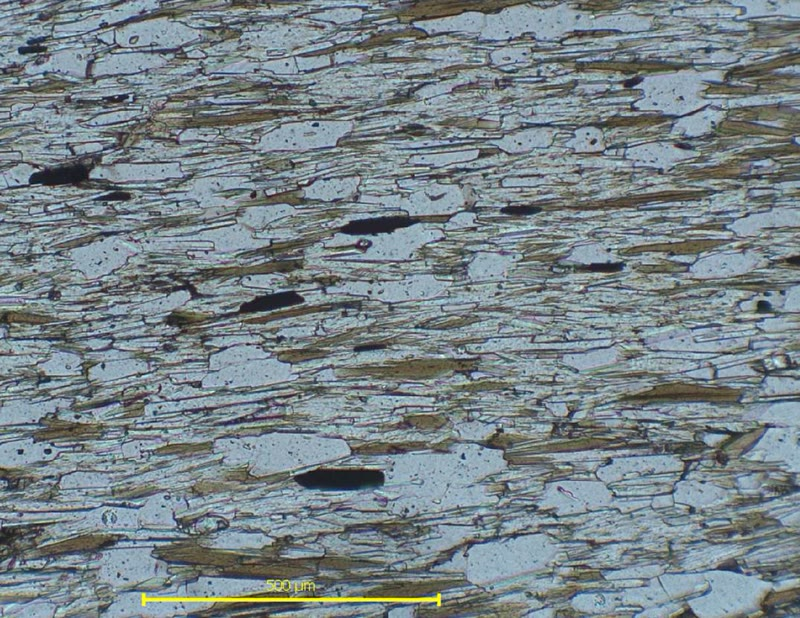
\includegraphics[height=4.3cm]{images/book2/g12-geoloshe-slaty-cleavage.jpg}\hspace{0.03\linewidth}%
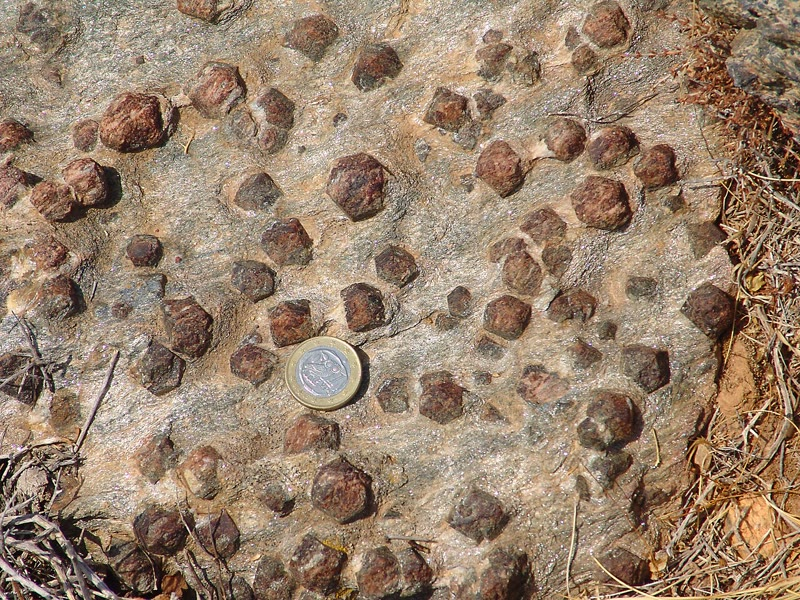
\includegraphics[height=4.3cm]{images/book2/g12-churchard-syros-garnet-schist.jpg}

\smallskip
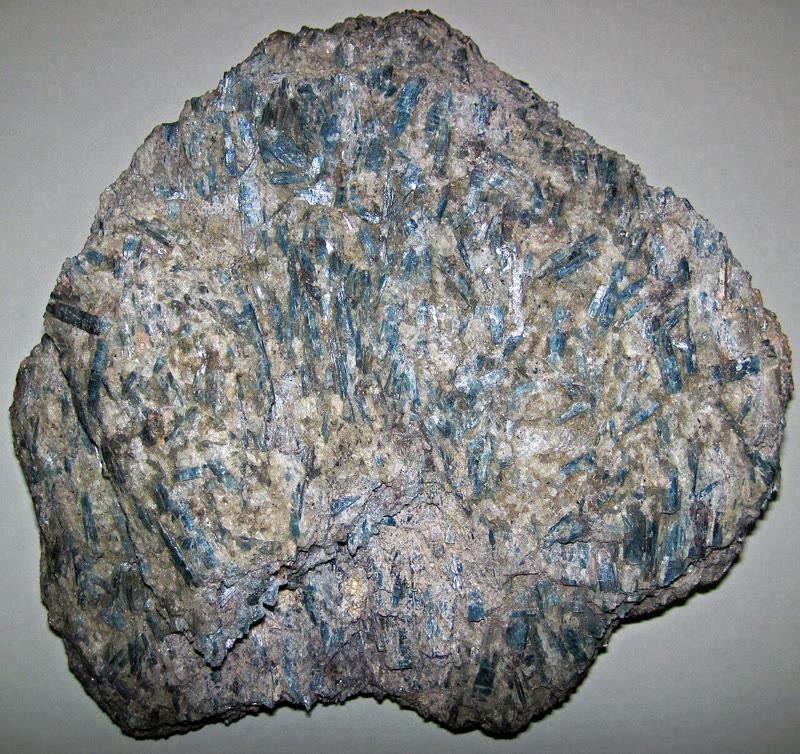
\includegraphics[height=4.3cm]{images/book2/g12-stjohn-kyanite-schist.jpg}\hspace{0.03\linewidth}%
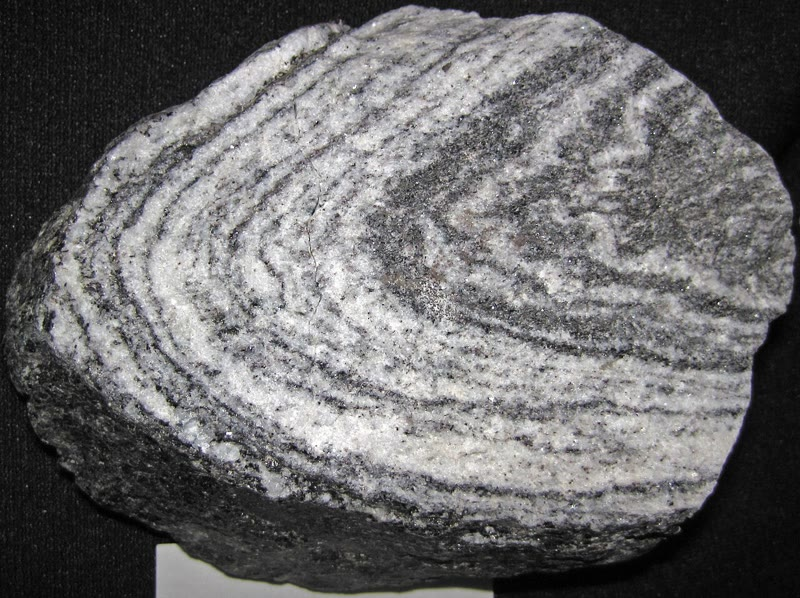
\includegraphics[height=4.3cm]{images/book2/g12-stjohn-gneiss.jpg}

{\small Top left: a slate under the microscope (the yellow bar is
\qty{500}{\micro\metre}): its flakes of mica all lie the same way.
Top right: a garnet mica schist on the island of Syros; the coin is
\qty{23}{mm} across. Bottom left: a schist with blue blades of kyanite.
Bottom right: a gneiss with bands of quartz (light) and of biotite mica
(dark). Photographs Geoloshe (CC0), Graeme Churchard (CC~BY~2.0) and James
St.~John (CC~BY~2.0).}
\end{omfigure}
% ledger: photo:g12-slaty-cleavage, photo:g12-syros-schist, photo:g12-kyanite-schist, photo:g12-gneiss

Along a typical \omterm{def:g11:lithosphere-asthenosphere:geotherm}{geotherm}, slate forms between about 5 and \qty{10}{km}
down, phyllite between 10 and 15, schist between 15 and 20, and gneiss between
20 and \qty{25}{km}; deeper still, the rock begins to melt in places. The
\omterm{def:g12:metamorphic-rocks:foliation}{foliation} records the direction of the squeeze: it forms across the
\omterm{def:g12:mountain-building:shortening}{shortening} that builds mountains (\cref{ch:g12:mountain-building}), and the
original layering of the mud may still be seen crossing it at an angle.
% ledger: earle:settings, earle:foliation

Rocks without flat or long minerals do not show a \omterm{def:g12:metamorphic-rocks:foliation}{foliation} even when they
are squeezed. A limestone becomes a \textbf{marble}, made of larger crystals
of calcite in which the fossils have been wiped out; a sandstone becomes a
\textbf{quartzite}, whose quartz grains have grown into one another; and a
mud heated without being squeezed becomes a hard, fine-grained rock without
\omterm{def:g12:metamorphic-rocks:foliation}{foliation}, a \textbf{hornfels}.
% ledger: earle:foliation, earle:contact

\section{Contact and regional metamorphism}

\begin{definition}[Contact metamorphism; regional metamorphism; aureole]\label{def:g12:metamorphic-rocks:contact-regional}
\emph{Contact metamorphism}\index{contact metamorphism} is the \omterm{def:g12:metamorphic-rocks:metamorphism}{metamorphism}
of rocks heated by a body of magma that has intruded them; it is confined to
a zone around the \omterm{def:g11:igneous-rocks:intrusion}{intrusion}, its \emph{aureole}\index{aureole}, in which the
grade rises towards the contact. \emph{Regional
metamorphism}\index{regional metamorphism} affects rocks buried deep over
large regions, usually where plates converge; the rocks are squeezed as well
as heated, and are almost always foliated.
\end{definition}
% ledger: earle:contact, earle:regional, tulane:metamorphism

\subsection{Around a body of magma}

A body of magma at about \qty{1000}{\celsius} that rises into the cold upper
crust heats the rocks around it. Their temperature can reach 300 to more
than \qty{800}{\celsius}, at the low pressures of shallow depths. The
\omterm{def:g12:metamorphic-rocks:contact-regional}{aureole} is narrow: a few centimetres around a thin sheet of magma, up to
several tens of metres around a large body. Its rocks are heated without
being squeezed, so they are not foliated: mud becomes hornfels, limestone
marble, sandstone quartzite. A body of magma that settles deep in rocks that
are already hot makes hardly any \omterm{def:g12:metamorphic-rocks:contact-regional}{aureole}.
% ledger: earle:contact, earle:settings (magma bodies around 1000 degC)

\begin{omfigure}
\begin{tikzpicture}[font=\scriptsize]
  \def\pluton{(3.0,0) .. controls (3.0,2.3) and (7.0,2.3) .. (7.0,0) -- cycle}
  \def\aureole{(2.45,0) .. controls (2.45,2.95) and (7.55,2.95) .. (7.55,0) -- cycle}
  \fill[lith sandstone] (0,0) rectangle (10,0.8);
  \fill[lith limestone] (0,0.8) rectangle (10,1.6);
  \fill[lith shale] (0,1.6) rectangle (10,3);
  \fill[omThm, opacity=0.30] \aureole;
  \draw[omThm, line width=0.6pt, dashed] (2.45,0) .. controls (2.45,2.95) and (7.55,2.95) .. (7.55,0);
  \fill[lith granite] \pluton;
  \draw[black!70, line width=0.6pt] (3.0,0) .. controls (3.0,2.3) and (7.0,2.3) .. (7.0,0);
  \draw[black!60] (0,0) rectangle (10,3);
  \node[fill=white, inner sep=1.5pt] at (5,0.45) {granite (once magma)};
  \draw[black!70] (6.0,1.95) -- (10.6,2.4) node[right] {hornfels, from mud};
  \draw[black!70] (7.0,1.2) -- (10.6,1.2) node[right] {marble, from limestone};
  \draw[black!70] (7.25,0.4) -- (10.6,0.4) node[right] {quartzite, from sandstone};
  \node[left] at (0,2.3) {shale};
  \node[left] at (0,1.2) {limestone};
  \node[left] at (0,0.4) {sandstone};
  \draw[omThm] (4.2,2.05) -- (3.4,3.25) node[above, omThm] {aureole};
\end{tikzpicture}

{\small \omterm{def:g12:metamorphic-rocks:contact-regional}{Contact metamorphism}, in cross-section: a body of magma has risen
into layered sedimentary rocks and heated a narrow \omterm{def:g12:metamorphic-rocks:contact-regional}{aureole} (red) around it,
whose rocks recrystallise without being squeezed. Schematic: real \omterm{def:g12:metamorphic-rocks:contact-regional}{aureoles}
are centimetres to tens of metres wide.}
\end{omfigure}
% ledger: earle:contact

\subsection{Under a mountain belt}

\omterm{def:g12:metamorphic-rocks:contact-regional}{Regional metamorphism} needs burial to 10 or \qty{20}{km}, so it affects
thousands of square kilometres at once. The likeliest place is the \omterm{def:g12:continental-crust:root}{root} of a
mountain belt, where collision thickens the crust and pushes its rocks down
(\cref{ch:g12:mountain-building}). In one old belt whose zones have been
mapped, the rocks of the sillimanite zone were heated above
\qty{700}{\celsius} and buried 20 to \qty{25}{km} deep, while those of the
outer chlorite zone were probably never buried more than about \qty{5}{km}.
The mountains above were then worn down over tens of millions of years; as
the load was removed, the thick crust rose again, and the once-deep zones now
lie at the surface (\cref{ch:g12:destruction-of-mountains}).
% ledger: earle:regional

\subsection{Three geotherms}

The \omterm{def:g12:metamorphic-rocks:polymorph}{polymorphs} show at a glance that the same depth does not mean the same
rock everywhere: it depends on the \omterm{def:g11:lithosphere-asthenosphere:geotherm}{geotherm}. The figure of the \omterm{def:g12:metamorphic-rocks:polymorph}{polymorphs}
carries three of them.
% ledger: earle:settings

\begin{itemize}
  \item A \textbf{typical} \omterm{def:g11:lithosphere-asthenosphere:geotherm}{geotherm}, about \qty{30}{\celsius} per
        kilometre: the temperature reaches about \qty{300}{\celsius} at
        \qty{10}{km}. It passes beneath the triple point, so kyanite gives
        way directly to sillimanite, at about \qty{574}{\celsius} and
        \qty{18.8}{km}.
  \item A \omterm{def:g11:lithosphere-asthenosphere:geotherm}{geotherm} of a \textbf{volcanic area}, 40 to \qty{50}{\celsius} per
        kilometre, steepened by the heat of rising magma: the rocks reach
        high temperatures at shallow depths. At \qty{50}{\celsius} per
        kilometre, andalusite appears at about \qty{6.6}{km} and gives way to
        sillimanite at about \qty{10.9}{km}, \qty{553}{\celsius}.
  \item The \omterm{def:g11:lithosphere-asthenosphere:geotherm}{geotherm} of a \textbf{\omterm{def:g11:subduction-zones:subduction}{subduction zone}}, under
        \qty{10}{\celsius} per kilometre: the \omterm{def:g11:ocean-ridges:oceanic-lithosphere}{oceanic crust} carried down
        stays several hundred degrees colder than the mantle around it. At
        \qty{36}{km} it is only about \qty{370}{\celsius}, deep in the
        kyanite field. This is the cold, high-pressure path on which basalt
        becomes \omterm{def:g11:subduction-zones:eclogite}{blueschist}, then \omterm{def:g11:subduction-zones:eclogite}{eclogite}, at about \qty{35}{km}.
\end{itemize}
% values: cross_30_0 573.6 degC 18.79 km; cross_50_0 340.1 degC 6.60 km; cross_50_1 553.0 degC 10.86 km; sub10_T_at_1gpa 370.2 (al2sio5.py)
% ledger: earle:settings

So each metamorphic rock carries a record of the \omterm{def:g11:lithosphere-asthenosphere:geotherm}{geotherm} under which it
formed, and of the plate setting behind it: andalusite and hornfels point to
heat at shallow depths, around bodies of magma; kyanite and sillimanite
schists and gneisses to the deep \omterm{def:g12:continental-crust:root}{roots} of mountain belts; \omterm{def:g11:subduction-zones:eclogite}{blueschists} and
\omterm{def:g11:subduction-zones:eclogite}{eclogites} to \omterm{def:g11:subduction-zones:subduction}{subduction zones}. Most of these rocks could only be seen
because they came back to the surface without changing back. As they rise
and cool, their reactions slow down, and the water that the reverse
reactions would need has escaped on the way down.
% ledger: earle:settings, earle:contact, tulane:metamorphism (retrograde metamorphism uncommon)

\section{Exercises}

\begin{exercise}[$\star$]\label{exo:g12:metamorphic-rocks:1}
Give the word: (a) minerals with the same composition but different crystal
structures; (b) the line on a map where an \omterm{def:g12:metamorphic-rocks:index-mineral}{index mineral} first appears;
(c) the zone of heated rocks around a body of magma; (d) the parallel planes
made by aligned flat minerals; (e) the pressure due to the weight of the
rocks above.
\end{exercise}

\begin{exercise}[$\star$]\label{exo:g12:metamorphic-rocks:2}
Name the metamorphic rock that each \omterm{def:g10:soil-formation:weathering-profile}{parent rock} becomes: (1) a limestone;
(2) a sandstone; (3) a mud, at low grade under a squeeze; (4) a mud, at high
grade; (5) a mud, heated by a body of magma without being squeezed.
\end{exercise}

\begin{exercise}[$\star$]\label{exo:g12:metamorphic-rocks:3}
With $\rho = \qty{2830}{kg/m^3}$ and $g = \qty{9.81}{m/s^2}$, compute the
\omterm{def:g12:metamorphic-rocks:lithostatic}{lithostatic pressure}, in \unit{GPa}, at \qty{10}{km} and at \qty{20}{km}.
\end{exercise}

\begin{exercise}[$\star$]\label{exo:g12:metamorphic-rocks:4}
On the diagram of the \omterm{def:g12:metamorphic-rocks:polymorph}{polymorphs} of \ce{Al2SiO5}, which mineral is stable
(1) at \qty{400}{\celsius} and \qty{0.6}{GPa}; (2) at \qty{500}{\celsius}
and \qty{0.2}{GPa}; (3) at \qty{750}{\celsius} and \qty{0.3}{GPa}?
\end{exercise}

\begin{exercise}[$\star$]\label{exo:g12:metamorphic-rocks:5}
(1) Put in order of rising grade: schist, slate, gneiss, phyllite. (2) In
which of them can the micas be seen with the naked eye? (3) Which one shows
light and dark bands?
\end{exercise}

\begin{exercise}[$\star\star$]\label{exo:g12:metamorphic-rocks:6}
(1) Compute the \omterm{def:g12:metamorphic-rocks:lithostatic}{lithostatic pressure} at the base of a crust \qty{35}{km}
thick ($\rho = \qty{2830}{kg/m^3}$) and express it in atmospheres
($\qty{1}{atm} = \qty{101325}{Pa}$). (2) Compute the pressure on the floor
of an ocean \qty{4}{km} deep, with sea water of density
\qty{1025}{kg/m^3}. (3) How many times larger is the first?
\end{exercise}

\begin{exercise}[$\star\star$]\label{exo:g12:metamorphic-rocks:7}
The triple point of \ce{Al2SiO5} lies at \qty{504}{\celsius} and
\qty{0.375}{GPa}. (1) At what depth is that pressure reached ($\rho =
\qty{2830}{kg/m^3}$)? (2) What \omterm{def:g11:lithosphere-asthenosphere:geotherm}{geothermal gradient}, starting from
\qty{10}{\celsius} at the surface, passes exactly through it? (3) Is a rock
that holds all three \omterm{def:g12:metamorphic-rocks:polymorph}{polymorphs} likely to be common?
\end{exercise}

\begin{exercise}[$\star\star$]\label{exo:g12:metamorphic-rocks:8}
In the photograph of the garnet schist of Syros, the largest garnets are
about a third of the coin across, which is \qty{23}{mm}. (1) Estimate
their diameter. (2) If a garnet's diameter grows by about \qty{1}{mm} in a
million years, how long did they take to grow? (3) What does that tell you
about the time a rock spends at depth?
\end{exercise}

\begin{exercise}[$\star\star$]\label{exo:g12:metamorphic-rocks:9}
Walking \qty{24}{km} westward across an old mountain belt, a geologist
records rocks made from mud. At the start they hold chlorite and biotite
only; the first garnet appears after \qty{6}{km}, the first staurolite after
\qty{11}{km}, the first kyanite after \qty{15}{km}, the first sillimanite
after \qty{20}{km}. (1) How many \omterm{def:g12:metamorphic-rocks:index-mineral}{isograds} were crossed? Name them in order.
(2) In which direction does the grade rise? (3) Where were the rocks buried
deepest, and roughly how hot did they become there?
\end{exercise}

\begin{exercise}[$\star\star$]\label{exo:g12:metamorphic-rocks:10}
A body of magma rises into layers of mud, limestone and sandstone near the
surface. (1) Name the rock each layer becomes next to it. (2) Why are these
rocks not foliated? (3) A second body of magma settles \qty{20}{km} down, in
rocks already near \qty{500}{\celsius}. Why does it make hardly any \omterm{def:g12:metamorphic-rocks:contact-regional}{aureole}?
\end{exercise}

\begin{exercise}[$\star\star$]\label{exo:g12:metamorphic-rocks:11}
A layer of mud is squeezed from the east and the west during a collision,
and grows micas as it is heated. (1) How do the micas lie: their flat faces
facing east--west or north--south? (2) Is the \omterm{def:g12:metamorphic-rocks:foliation}{foliation} that forms
horizontal or vertical? (3) A marble and a quartzite squeezed in the same
way show no \omterm{def:g12:metamorphic-rocks:foliation}{foliation}. Why?
\end{exercise}

\begin{exercise}[$\star\star\star$]\label{exo:g12:metamorphic-rocks:12}
Between 500 and \qty{700}{\celsius}, the kyanite--sillimanite boundary is
close to the straight line $P = 0.577 + 0.00209\,(T - 600)$, with $P$ in
\unit{GPa} and $T$ in \unit{\celsius}. A typical \omterm{def:g11:lithosphere-asthenosphere:geotherm}{geotherm} is $T = 10 + 30z$
($z$ in \unit{km}), and $P = 0.0278\,z$. (1) Write the \omterm{def:g11:lithosphere-asthenosphere:geotherm}{geotherm} as $P$ as a
function of $T$. (2) Find where it crosses the boundary: temperature, pressure,
depth. (3) Along this \omterm{def:g11:lithosphere-asthenosphere:geotherm}{geotherm}, which \omterm{def:g12:metamorphic-rocks:polymorph}{polymorph} is stable just above that
depth, and which just below?
\end{exercise}

\begin{exercise}[$\star\star\star$]\label{exo:g12:metamorphic-rocks:13}
(1) Along a \omterm{def:g11:subduction-zones:subduction}{subduction} \omterm{def:g11:lithosphere-asthenosphere:geotherm}{geotherm} of \qty{10}{\celsius} per kilometre, starting
from \qty{10}{\celsius}, what is the temperature at \qty{35}{km}, where
\omterm{def:g11:subduction-zones:eclogite}{eclogite} forms? (2) What is it along a typical \omterm{def:g11:lithosphere-asthenosphere:geotherm}{geotherm} of
\qty{30}{\celsius} per kilometre? (3) Place both points on the diagram of
the \omterm{def:g12:metamorphic-rocks:polymorph}{polymorphs}: which \omterm{def:g12:metamorphic-rocks:polymorph}{polymorph} is stable at the first? (4) Why do
\omterm{def:g11:subduction-zones:eclogite}{blueschists} and \omterm{def:g11:subduction-zones:eclogite}{eclogites} form in \omterm{def:g11:subduction-zones:subduction}{subduction zones} and hardly anywhere else?
\end{exercise}

\begin{exercise}[$\star\star\star$]\label{exo:g12:metamorphic-rocks:14}
The densities of kyanite, sillimanite and andalusite are \num{3.61},
\num{3.24} and \qty{3.15}{g/cm^3}. (1) Compute the volume of \qty{1}{kg} of
each, in \unit{cm^3}. (2) By what percentage is kyanite smaller than
andalusite of the same mass? (3) Explain, with the idea that a high pressure
favours the arrangement that takes the least room, why kyanite holds the
high-pressure field of the diagram.
\end{exercise}

\begin{exercise}[$\star\star\star$]\label{exo:g12:metamorphic-rocks:15}
In an old mountain belt, the rocks of the sillimanite zone were heated above
\qty{700}{\celsius} and buried 20 to \qty{25}{km} deep. (1) Compute the
pressure at 20 and at \qty{25}{km}. (2) Using the line of
exercise~12, find the lowest temperature at which sillimanite is stable at
each of these pressures. Is \qty{700}{\celsius} consistent with sillimanite?
(3) What \omterm{def:g11:lithosphere-asthenosphere:geotherm}{geothermal gradients}, from \qty{10}{\celsius} at the surface, does
\qty{700}{\celsius} at 20 and at \qty{25}{km} imply? (4) The rocks were
exposed at the surface about 40 million years later. At what mean rate was
the rock above them removed, in \unit{mm} a year?
\end{exercise}

\begin{problem}[{Weekend problem --- The history of a kyanite schist}]
\label{pb:g12:metamorphic-rocks:1}
% ledger: hm93:table11, cm95:crust, earle:controls, earle:settings, earle:regional, tulane:roots, tulane:metamorphism, iugs:barrow; Book 3: webmineral:polymorphs; Book 1: ussa76:sea-level
% values: pb_z_km 25.214, pb_grad 23.4, pb_kysil_P_at_600_gpa 0.577 (al2sio5.py); t_on_kysil(7.0) = 658.9
A schist collected in the core of an old mountain belt holds muscovite,
biotite, quartz, garnets up to \qty{8}{mm} across, and blue blades of
kyanite; it holds neither sillimanite nor andalusite. Laboratory analyses of
its garnet and biotite give the conditions under which it crystallised:
about \qty{600}{\celsius} and \qty{0.70}{GPa}. Take $\rho =
\qty{2830}{kg/m^3}$, $g = \qty{9.81}{m/s^2}$, \qty{10}{\celsius} at the
surface, and the kyanite--sillimanite line of exercise~12, $P = 0.577 +
0.00209\,(T - 600)$.

\medskip
\noindent\textbf{Part I --- The minerals.}
\begin{enumerate}
  \item Why is the rock called a schist? Which of its minerals make the
        \omterm{def:g12:metamorphic-rocks:foliation}{schistosity}?
  \item Kyanite, andalusite and sillimanite share one formula. Write it, and
        give the word for such minerals.
  \item The densities of kyanite and andalusite are \num{3.61} and
        \qty{3.15}{g/cm^3}. By what percentage is the volume of a kilogram of
        kyanite smaller? Which one does pressure favour?
  \item In the sequence of \omterm{def:g12:metamorphic-rocks:index-mineral}{index minerals} of rocks made from mud, which zone
        does the rock belong to? Which \omterm{def:g12:metamorphic-rocks:index-mineral}{isograds} did it cross on its way down?
  \item If the garnets' diameter grew by about \qty{1}{mm} in a million
        years, how long did the largest ones take to grow?
\end{enumerate}

\medskip
\noindent\textbf{Part II --- Pressure and temperature.}
\begin{enumerate}[resume]
  \item At \qty{600}{\celsius}, above what pressure is kyanite stable rather
        than sillimanite?
  \item Check that the point (\qty{600}{\celsius}, \qty{0.70}{GPa}) lies in
        the kyanite field.
  \item The missing sillimanite gives a lowest pressure at
        \qty{600}{\celsius}. What is it?
  \item Had the rock been heated further at \qty{0.70}{GPa}, at what
        temperature would its kyanite have turned into sillimanite?
  \item Express \qty{0.70}{GPa} in kilobars ($\qty{1}{kbar} =
        \qty{e8}{Pa}$) and in atmospheres ($\qty{1}{atm} = \qty{101325}{Pa}$).
\end{enumerate}

\medskip
\noindent\textbf{Part III --- The burial depth.}
\begin{enumerate}[resume]
  \item By how many megapascals does the \omterm{def:g12:metamorphic-rocks:lithostatic}{lithostatic pressure} rise per
        kilometre?
  \item At what depth was the schist when it crystallised?
  \item What is the smallest depth allowed by the missing sillimanite
        (question 8)?
  \item Redo question 12 with a density of \qty{2700}{kg/m^3} for the rocks
        above. By what percentage does the depth change?
  \item A \omterm{def:g12:continental-crust:continental-crust}{continental crust} is normally 35 to \qty{40}{km} thick, and 50 to
        \qty{70}{km} under mountain belts. Did the schist crystallise in the
        crust or in the mantle?
\end{enumerate}

\medskip
\noindent\textbf{Part IV --- The geotherm, and the way back up.}
\begin{enumerate}[resume]
  \item What mean \omterm{def:g11:lithosphere-asthenosphere:geotherm}{geothermal gradient} do \qty{600}{\celsius} at that depth
        imply?
  \item Compare it with the gradients of a \omterm{def:g11:subduction-zones:subduction}{subduction zone}, a typical
        crust and a volcanic area. Which kind of \omterm{def:g12:metamorphic-rocks:metamorphism}{metamorphism} made the rock?
  \item Along a typical \omterm{def:g11:lithosphere-asthenosphere:geotherm}{geotherm} of \qty{30}{\celsius} per kilometre, what
        would the temperature be at the depth of question 12? Which
        \omterm{def:g12:metamorphic-rocks:polymorph}{polymorph} would then be stable at \qty{0.70}{GPa}?
  \item To bring the schist to the surface, all the rock above it had to be
        removed. At a mean rate of \qty{0.5}{mm} a year, how long did that
        take?
  \item Why did the kyanite not turn back into andalusite on the way up?
  \item Sum up: at what depth did this kyanite schist crystallise?
\end{enumerate}
\end{problem}
